\documentclass{article}
\usepackage{graphicx}
\usepackage[]{mdframed}
\usepackage{tabularx}
\usepackage{subfig}
\usepackage{placeins}
\usepackage{float}
\usepackage{parskip}

\graphicspath{ {./graphing/} }
\usepackage[a4paper, total={6in, 8in}]{geometry}

\newcolumntype{Y}{>{\centering\arraybackslash}X}

\author{Sidharth Babu, SNB2593 \and Tianda Huang, TH32684}
\title{ECE 361E: Homework 4}

\begin{document}
\begin{mdframed}
    \maketitle
\end{mdframed}
\pagebreak

\section*{Problem 1}
\subsection*{Question 2}
\begin{figure}[!htb]
    \caption{\textit{Table 1}}
    \begin{tabularx}{\textwidth}{|*{7}{Y|}}
        \hline
        Model       & Training Accuracy [\%] & Test Accuracy [\%] & Total Time for Training [s] & Number of Trainable Params\\
        \hline
        VGG11       & 99.69  & 78.25  & 773.210  & 9,750,922 \\
        \hline
        VGG16       & 99.69  & 77.64  & 1223.664 & 14,655,050\\
        \hline
        MobileNet   & 99.30  & 79.41  & 1186.733 & 3,217,226 \\
        \hline
    \end{tabularx}
    \label{fig:model-summary}
\end{figure}

\subsection*{Question 3}
\begin{figure}[!htb]
    \centering
    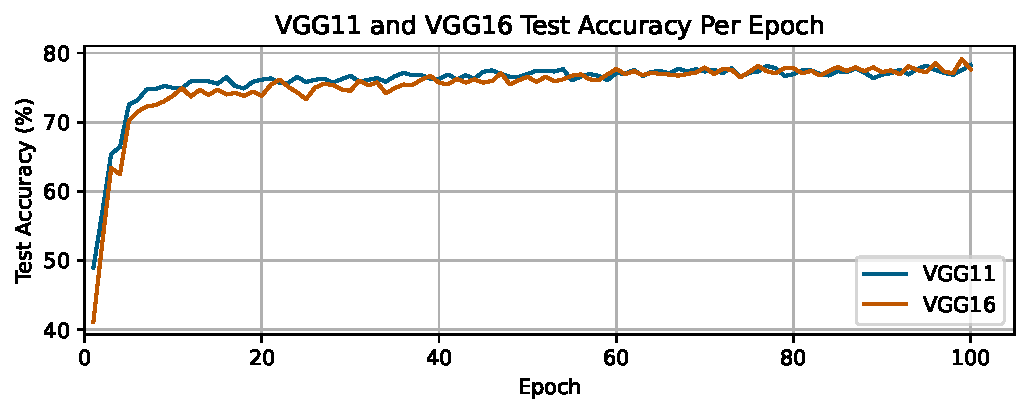
\includegraphics[width=\textwidth]{vgg11_16_acc.pdf}
    \caption{Test Accuracy of VGG11 and VGG16}
    \label{fig:vgg-epoch-accuracy}
\end{figure}


\clearpage\pagebreak
\section*{Problem 2}
\subsection*{Question 2}
\begin{figure}[!htb]
    \caption{\textit{Table 2}}
    \begin{tabularx}{\textwidth}{|*{7}{Y|}}
        \hline
        & \multicolumn{2}{c|}{Total Inference Time [s]}  & \multicolumn{2}{c|}{RAM memory [MB]} & \multicolumn{2}{c|}{Accuracy [\%]} \\
        \cline{1-7}
                    & MC1       & RPi       & MC1   & RPi   & MC1   & RPi \\
        \hline
        VGG11       & 648.79    & 582.19    & 306   & 155   & 78.25 & 78.25 \\
        \hline
        VGG16       & 1063.83   & 1004.81   & 325   & 174   & 77.64 & 77.64 \\
        \hline
        MobileNet   & 495.46    & 199.86    & 282   & 128   & 79.41 & 79.41 \\
        \hline
    \end{tabularx}
    \label{fig:deploy-summary}
\end{figure}

\subsection*{Question 3}
\begin{figure}[!htb]
    \centering
    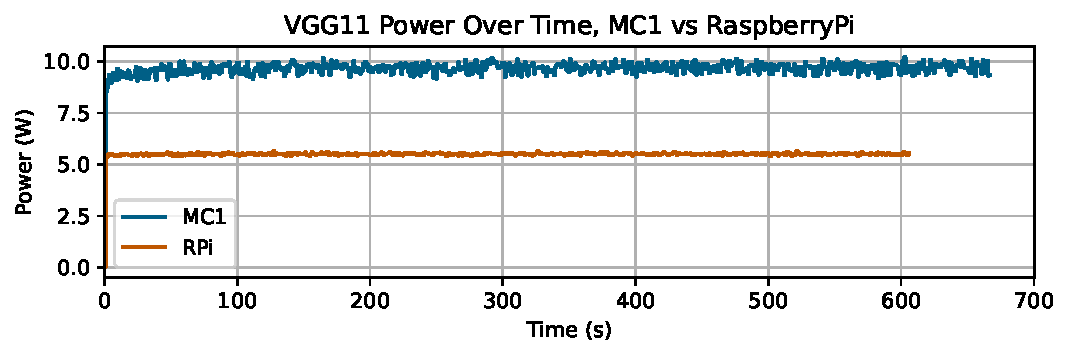
\includegraphics[width=\textwidth]{vgg11_power.pdf}
    \caption{}
    \label{fig:vgg11-power}
\end{figure}

\begin{figure}[!htb]
    \centering
    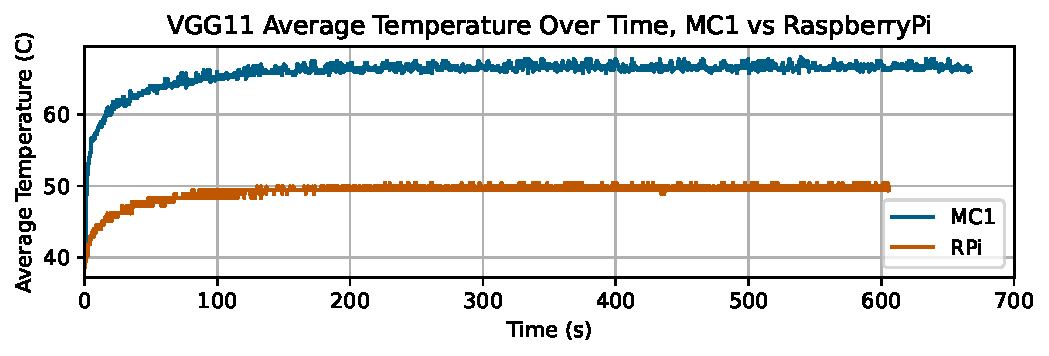
\includegraphics[width=\textwidth]{vgg11_average_temperature.pdf}
    \caption{}
    \label{fig:vgg11-avg-temp}
\end{figure}
\clearpage
\begin{figure}[!htb]
    \caption{\textit{Table 3}}
    \begin{tabularx}{\textwidth}{|c|*{2}{Y|}}
        \hline
        Model     & MC1 Total Energy Consumption [J] & RPi total Energy Consumption [J] \\
        \hline
        VGG11     & 6442.54   & 3330.53 \\
        \hline
        VGG16     & 10847.49  & 5675.75  \\
        \hline
        MobileNet & 3957.77   & 1168.07 \\
        \hline
    \end{tabularx}
    \label{fig:deploy-energy}
\end{figure}

\section*{Problem 3}
\subsection*{BONUS}
In order to properly discuss the tradeoffs between the two deployment frameworks, first we must include the data that we profiled with the same models
on ONNX.

\begin{figure}[!htb]
    \caption{\textit{Table 4 - ONNX Model Summary}}
    \begin{tabularx}{\textwidth}{|*{7}{Y|}}
        \hline
        Model & Training Accuracy [\%] & Test Accuracy [\%] & Total Time for Training [s] & Number of Trainable Params \\
        \hline
        VGG11 & 97.57 & 76.48 & 3011.79 & 9,750,922   \\
        \hline
        VGG16 & 97.86 & 78.89 & 3622.42 & 14,655,050   \\
        \hline
        MobileNet & 99.42 & 77.75 & 2211.56 & 3,217,226 \\
        \hline
    \end{tabularx}
    \label{fig:model-summary-onnx}
\end{figure}

\begin{figure}[!htb]
    \caption{\textit{Table 5 - ONNX Deployment Summary}}
    \begin{tabularx}{\textwidth}{|*{7}{Y|}}
        \hline
        & \multicolumn{2}{c|}{Total Inference Time [s]}  & \multicolumn{2}{c|}{RAM memory [MB]} & \multicolumn{2}{c|}{Accuracy [\%]} \\
        \cline{1-7}
        & MC1 & RPi & MC1 & RPi & MC1 & RPi \\
        \hline
        VGG11 & 658.23 & 680.61 & 330 & 171 & 76.48 & 76.48\\
        \hline
        VGG16 & 990.92 & 1172.02 & 352 & 192 & 78.89 & 78.89\\
        \hline
        MobileNet & 491.65 & 329.30 & 302 & 139 & 77.75 & 77.75\\
        \hline
    \end{tabularx}
    \label{fig:deploy-summary-onnx}
\end{figure}

\begin{figure}[!htb]
    \caption{\textit{Table 6 - ONNX Energy Summary}}
    \begin{tabularx}{\textwidth}{|c|*{2}{Y|}}
        \hline
        Model & MC1 Total Energy Consumption [J] & RPi total Energy Consumption [J] \\
        \hline
        VGG11 & 6574.78 & 3739.40 \\
        \hline
        VGG16 & 10106.79 & 6381.64 \\
        \hline
        MobileNet & 4196.58 & 1877.45 \\
        \hline
    \end{tabularx}
    \label{fig:deploy-energy-onnx}
\end{figure}

Overall, the TF deployment is more efficient based on our data. 

Looking at subsection 1 of tables 5 and 2, we can see that the TF Deployment has lower inference times than the ONNX deployment in all cases except for VGG16-MC1 and MobileNet-MC1. This could be due to some particular hardware feature of the MC1 that the ONNX framework optimizes better for. It could also be spurious data, and repeating this experiment may be necessary to confirm this either way.

In subsection 2 of tables 5 and 2, we can see that the TF deployment uses less RAM in all cases. This could be due to a variety of reasons, but could indicate that TF's memory footprint is generally be better than ONNX's. In order to properly confirm this, additional models would have to be tested on both frameworks, and on more hardware platforms.

In tables 3 and 6, we can see that the TF deployment uses less energy in all cases besides the VGG16-MC1. Since this is an outlier, it may be that this data point is spurious, but it would need to be confirmed through additionalruns of the experiment.

With these comparisons on our data, we can see that Tensorflow Lite seems to perform better in all three key metrics. Therefore, we would claim that Tensorflow is the more efficient deployment framework. 

In terms of preference, the ONNX and TFLITE frameworks both present their own advantages. ONNX may generally be better for R\&D purposes, as it is more flexible, and does not restrict the user to a particular model training framework. However, for production deployment at scale, TFLITE is likely the better choice, as we have shown that it is generally more efficient.


\section*{Contributions and Valuable Things Learned}
Both group members, Sidharth Babu and Tianda Huang, contributed an equal amount of work due to working on the entire project together.

\end{document}